\documentclass{exmppr}
\usepackage{tasks}
\usepackage{tikz}
\usepackage{epigraph}
\usepackage{enumerate}

\institutename{Sardar Vallabhbhai National Institute of Technology, Surat}
\sem{1}%which semester
\coursename{Distributed Computing}%name of course
\ccode{CO601}%course code
\type{MidSem}%endsem or midsemm
\season{Summer}%winter, fall, summer, etc.
\batch{2018-19}% batch 2013-14,2014-15,2015-16 etc

\profname{Udai P Rao \& Bavesh N Gohil}%name of prof

\newtheorem{exercise}{\bfseries}

\begin{document}
\begin{enumerate}

\item \begin{enumerate}
\item Why distribution is required? Clearly indicate your answer with set of reasons. Also enlist the problems faced because of distribution.

\item Differentiate between preemptive and non-preemptive precess migration. Which one is mostly possible in receiver initiated scheduling algorithm?

\item It is considered that all three approached of location policy of sender-initiated algorithms cause system instability at high system loads. Present you reasoning with valid statement.
\end{enumerate}
\item \begin{enumerate}
\item Present a comparison among \textit{distributed OS, Network OS and Middleware-based OS}. Use the following parameters: Degree of Transparency, Same OS on all nodes, Number of copies of OS, Basis for communication, Resource Management, Scalability, and Openness.

\item What do you mean by Secure multi-party Computation(SMC)? Present a scenario for secure multi-party computation to calculate average salary of employees of a company. Develop a protocol which should not reveal the individual's private information to any other employee during computation. Let us assume that the SMC for above application is restricted to four employees.
\end{enumerate}
\item \begin{enumerate}
\item Differentiate between RPC and RMI.

\item Explain following message communications with example: Persistent Synchronous, Transient Synchronous(delivery based).

\item Define the following terms: hit rate, latency, clock skew, clock drift

\item Explain Unix file sharing semantic with example.

\item Define ``has happened before relation($<$)". Write down the Lamport's clock and vector clock value at each event in the following diagram.
\end{enumerate}
\end{enumerate}

\centering
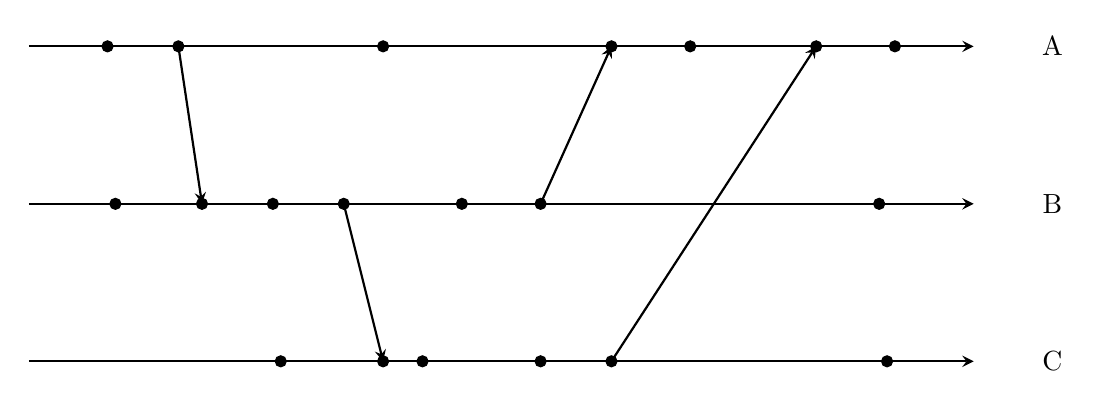
\begin{tikzpicture}[scale=1]
\draw[->,>=stealth,thick] (-4,0) -- (8,0) ;
\filldraw (-3,4) circle (2pt);
\filldraw (-2.1,4) circle (2pt);
\filldraw (.5,4) circle (2pt);
\filldraw (3.4,4) circle (2pt);
\filldraw (4.4,4) circle (2pt);
\filldraw (6,4) circle (2pt);
\filldraw (7,4) circle (2pt);

\draw[->,>=stealth,thick] (-4,2) -- (8,2) ;
\filldraw (-2.9,2) circle (2pt);
\filldraw (-1.8,2) circle (2pt);
\filldraw (-.9,2) circle (2pt);
\filldraw (0,2) circle (2pt);
\filldraw (1.5,2) circle (2pt);
\filldraw (2.5,2) circle (2pt);
\filldraw (6.8,2) circle (2pt);

\draw[->,>=stealth,thick] (-4,4) -- (8,4) ;
\filldraw (-0.8,0) circle (2pt);
\filldraw (0.5,0) circle (2pt);
\filldraw (1,0) circle (2pt);
\filldraw (2.5,0) circle (2pt);
\filldraw (3.4,0) circle (2pt);
\filldraw (6.9,0) circle (2pt);


\draw[->,>=stealth,thick] (-2.1,4) -- (-1.8,2) ;
\draw[->,>=stealth,thick] (0,2) -- (0.5,0) ;
\draw[->,>=stealth,thick] (2.5,2) -- (3.4,4) ;
\draw[->,>=stealth,thick] (3.4,0) -- (6,4) ;


\node (A) at (9, 4) {A};
\node (B) at (9, 2) {B};
\node (C) at (9, 0) {C};



\end{tikzpicture}

\newpage
\begin{center}\section*{Answers}\end{center}
%\input{sol1.tex}

\end{document}
